\documentclass[conference]{IEEEtran}
\IEEEoverridecommandlockouts
\usepackage{cite}
\usepackage{amsmath,amssymb}
\usepackage{graphicx}
\usepackage{booktabs}
\usepackage{array}
\usepackage[hidelinks]{hyperref}
\graphicspath{{figures/}}
\renewcommand{\arraystretch}{1.12}

\begin{document}

\title{Statistical Modelling of Packet-Loss Patterns in Computer Networks: Distribution Fitting, Burstiness Testing and Bayesian Estimation}

\author{
<<authors_tex>>
}

\maketitle

\begin{abstract}
Simple loss models treat every packet as an independent trial. Under that assumption, losses per second follow a Poisson law and the gaps between losses are exponential. We test this assumption on <<n_scen>> network conditions (wired broadband, campus Wi-Fi and a mobile hotspot). Each condition is generated from a two-state Gilbert-Elliott channel at <<rate>> packets per second for <<duration_h>> hour, giving <<packets>> packets per network. We fit Poisson, Negative Binomial, exponential and two-phase hyperexponential models by maximum likelihood and the EM algorithm. We test independence with the runs test and a Markov-chain likelihood-ratio test, and estimate loss rates with a Beta-Binomial model. The variance-to-mean ratio of losses per second is <<list_D>>, against 1 for a Poisson process, and the Poisson and exponential models are rejected in every case. A loss raises the chance of the next loss by a factor of <<amp_lo>> to <<amp_hi>>. Because of this dependence, nominal 95\% intervals for the loss rate cover the true value in only <<covN_lo>> to <<covN_hi>> of <<cov_reps>> simulated captures. Dividing the sample size by a design effect restores coverage to <<covA_lo>> to <<covA_hi>>. A power study shows that captures of at least ten minutes per network are needed for the measurement phase that follows.
\end{abstract}

\begin{IEEEkeywords}
packet loss, Gilbert-Elliott model, burstiness, goodness of fit, Bayesian estimation, design effect, Monte Carlo simulation
\end{IEEEkeywords}

\section{Introduction}
Voice calls, video streams and online games send small packets at a steady rate. Some of these packets never arrive. The share that is lost, the loss rate, is the figure most often used to describe a link. Operators quote it in service agreements, and protocol designers use it to set retransmission timers and the strength of forward error correction.

A loss rate on its own says little about how losses are arranged in time. Ten isolated losses can be hidden by a media decoder. Ten losses in a row cause a visible freeze. Textbook analysis usually assumes that each packet is lost independently with a fixed probability $p$. This makes the count of losses in a short window Binomial, close to Poisson, and the time between losses exponential. If losses cluster, both statements fail, and so do the standard errors built on them.

This paper studies how far the independence assumption breaks, how the breakdown can be measured, and what it costs for interval estimates of the loss rate. The work is organised in two phases. Phase 1, reported here, is a simulation study in which the true parameters of every network are known. This lets each estimator and test be checked against the truth before it is used on measured traces. Phase 2 will apply the same code to real captures.

Our contributions are as follows.
\begin{itemize}
\item We compare Poisson and Negative Binomial models for losses per second, and exponential and two-phase hyperexponential models for inter-loss gaps, with $\chi^2$, bootstrap Kolmogorov-Smirnov and AIC criteria.
\item We quantify dependence between consecutive packets with a runs test, a Markov-chain likelihood-ratio test and Bayesian estimates of the burst parameters.
\item We show by Monte Carlo simulation that naive intervals for the loss rate are over-confident, and that a design-effect correction brings coverage back near its nominal level.
\item We use a power study to set the capture length for the measurement phase.
\end{itemize}

Section~II reviews related work. Section~III describes the loss model and data. Section~IV sets out the statistical methods, and Section~V reports the results. Section~VI discusses limitations, and Section~VII concludes.

\section{Related Work}
Gilbert proposed a two-state Markov channel to describe burst errors on telephone lines \cite{gilbert1960}. Elliott extended it so that errors can occur in both states \cite{elliott1963}. The resulting Gilbert-Elliott model remains a standard description of bursty loss.

Early measurement work on the Internet found that losses are not independent. Bolot observed that probe packets sent close together tend to be lost together \cite{bolot1993}. Paxson analysed large sets of TCP transfers and reported correlated loss episodes \cite{paxson1997}. Yajnik et al. studied multicast traces and modelled the temporal dependence of loss with Markov chains of increasing order \cite{yajnik1999}. Jiang and Schulzrinne fitted Gilbert models to voice traffic and related burst length to perceived quality \cite{jiang2000}. Hasslinger and Hohlfeld discussed how the Gilbert-Elliott parameters can be estimated from traces for real-time services \cite{hasslinger2008}.

These studies concentrate on describing the loss process. Our focus is the statistical side: which standard tests detect the dependence, how much data they need, and how much the usual interval estimates mislead when dependence is ignored. For the last question we borrow the design effect from survey sampling \cite{kish1965}. For goodness of fit with estimated parameters we use the bootstrap form of the Kolmogorov-Smirnov test \cite{lilliefors1969,efron1993}.

\section{Loss Model and Data}
\subsection{Gilbert-Elliott channel}
The channel is in one of two hidden states, Good (G) or Bad (B). Before each packet it moves from G to B with probability $p$ and from B to G with probability $r$. A packet is lost with probability $h_G$ in the Good state and $h_B$ in the Bad state, where $h_G \ll h_B$. Balancing the flow between the two states gives the long-run share of time spent in Bad and the long-run loss rate:
\begin{equation}
\pi_B=\frac{p}{p+r},\qquad P(\text{loss})=(1-\pi_B)\,h_G+\pi_B\,h_B .
\label{eq:ge}
\end{equation}
The number of packets spent in each visit to a state is geometric, with mean $1/p$ in Good and $1/r$ in Bad.

\subsection{Scenarios and sampling}
Table~\ref{tab:params} lists the parameters of the <<n_scen>> scenarios. They were chosen to give low, medium and high loss with increasingly long Bad spells. Each scenario is a constant stream of <<rate>> packets per second, one every <<spacing_ms>>~ms, observed for <<duration_s>>~s. This gives <<packets>> packets per network and <<packets_total>> in total. All random draws use the seed <<seed>>, so every number in this paper can be reproduced.

\begin{table}[t]
\caption{Scenario parameters and the implied true loss rate}
\label{tab:params}
\centering
\footnotesize
\setlength{\tabcolsep}{3.2pt}
\begin{tabular}{lccccccc}
\toprule
Network & $p$ & $r$ & $h_G$ & $h_B$ & $\pi_B$ & Bad spell & True loss \\
\midrule
<<rows_params>>
\bottomrule
\end{tabular}
\\[2pt]
\raggedright\scriptsize Bad spell is the mean stay in Bad, $1/r$ packets. True loss follows from (\ref{eq:ge}).
\end{table}

\subsection{Simulation}
Stepping the chain one packet at a time is slow. We instead draw whole sojourn lengths from the geometric distribution, alternate the two states, and then mark each packet as lost with the loss probability of its state. This produces exactly the same process. From each trace we derive four data sets: losses per <<window_s>>-s window (<<windows>> counts), inter-loss gaps, burst lengths (runs of consecutive losses), and the four transition counts between delivered (N) and lost (L) packets. A uniform jitter inside each <<spacing_ms>>-ms slot turns packet indices into continuous loss times.

\section{Methodology}
\subsection{Distribution fitting}
For losses per window $x_1,\dots,x_n$ we fit a Poisson law, whose maximum-likelihood estimate is $\hat\lambda=\bar x$, and a Negative Binomial law,
\begin{align}
P(X=k)&=\binom{k+r_{\!NB}-1}{k}q^{r_{\!NB}}(1-q)^k,\\
\operatorname{Var}(X)&=\mu+\mu^2/r_{\!NB} .
\end{align}
The Negative Binomial is a Poisson law whose rate is Gamma distributed. It allows the variance to exceed the mean. We fit it by maximising the profile likelihood over $r_{\!NB}$ with the mean fixed at $\bar x$.

For inter-loss gaps we fit an exponential law, $\hat\lambda=1/\bar t$, and a two-phase hyperexponential mixture
\begin{equation}
f(t)=w\lambda_1e^{-\lambda_1t}+(1-w)\lambda_2e^{-\lambda_2t}.
\end{equation}
The fast phase $\lambda_1$ stands for gaps inside a burst and the slow phase $\lambda_2$ for gaps between bursts. The mixture is fitted with the EM algorithm \cite{dempster1977}. The E-step computes, for each gap, the posterior probability that it came from the fast phase. The M-step updates $w$, $\lambda_1$ and $\lambda_2$ as weighted maximum-likelihood estimates. Models are compared with $\text{AIC}=2k-2\ln L$ \cite{akaike1974}.

\subsection{Goodness of fit}
The Pearson statistic $\chi^2=\sum_i (O_i-E_i)^2/E_i$ compares observed and expected window counts. Tail bins are pooled until every expected count is at least 5, and the degrees of freedom are the number of bins minus one minus the number of fitted parameters. The index-of-dispersion test uses $(n-1)s^2/\bar x$, which follows $\chi^2_{n-1}$ under a Poisson law.

For the gaps we use the Kolmogorov-Smirnov distance $D=\sup_t|F_n(t)-F(t)|$. Because the rate is estimated from the same sample, the standard tables give p-values that are too large \cite{lilliefors1969}. We therefore build the null distribution by parametric bootstrap \cite{efron1993}: we simulate from the fitted model, refit, and recompute $D$, <<n_boot>> times for the exponential and <<n_boot_mix>> times for the mixture.

\subsection{Tests of independence}
The Wald-Wolfowitz runs test \cite{wald1940} counts the runs $R$ of identical outcomes in the 0/1 loss sequence. With $n_1$ losses and $n_0$ deliveries,
\begin{equation}
E[R]=\frac{2n_1n_0}{n}+1,\quad \operatorname{Var}(R)=\frac{2n_1n_0(2n_1n_0-n)}{n^2(n-1)} .
\end{equation}
Fewer runs than expected means that losses sit next to each other.

The Markov-chain test compares two models for the sequence. Under $H_0$ every packet is lost with the same probability. Under $H_1$ the probability depends on the previous packet: $a=P(L\mid N)$ and $b=P(L\mid L)$. With $n_{xy}$ the number of transitions from $x$ to $y$,
\begin{equation}
\hat a=\frac{n_{NL}}{n_{NN}+n_{NL}},\qquad \hat b=\frac{n_{LL}}{n_{LN}+n_{LL}},
\end{equation}
\begin{equation}
G^2=2(\ln L_1-\ln L_0).
\end{equation}
By Wilks' theorem \cite{wilks1938}, $G^2$ is approximately $\chi^2_1$ under $H_0$. The ratio $b/a$ measures how much one loss raises the chance of the next, and $1/(1-b)$ is the mean burst length.

To compare networks we use the Kruskal-Wallis test \cite{kruskal1952} on window counts, pairwise Mann-Whitney tests \cite{mann1947} with a Bonferroni correction, and a $\chi^2$ test of homogeneity on the table of lost and delivered packets. Rank tests are used because the counts are discrete, mostly zero and strongly skewed. All tests use $\alpha=<<alpha>>$.

\subsection{Bayesian estimation}
With a uniform $\text{Beta}(1,1)$ prior and $k$ losses in $n$ packets, the posterior of the loss probability is $\text{Beta}(1+k,\,1+n-k)$ \cite{gelman2013}. We report the posterior mean and the equal-tailed 95\% credible interval, show sequential updating for <<seq_label>>, and estimate the probability that the networks are ordered by loss rate from <<ord_draws>> posterior draws. The Markov parameters receive independent posteriors $a\sim\text{Beta}(1+n_{NL},1+n_{NN})$ and $b\sim\text{Beta}(1+n_{LL},1+n_{LN})$, which give credible intervals for $b/a$ and for the burst length. As a posterior predictive check, we compare the Beta-Binomial probability of at least <<heavy_k>> losses in one window, implied by the independent model, with the observed share of such windows.

\subsection{Design effect}
For a sum of correlated indicators,
\begin{equation}
\operatorname{Var}\Big(\sum_i X_i\Big)=\sum_i\operatorname{Var}(X_i)+2\sum_{i<j}\operatorname{Cov}(X_i,X_j).
\end{equation}
Inside a burst the covariances are positive, so the true variance of the loss count is larger than $np(1-p)$. Following Kish \cite{kish1965}, we split each trace into blocks of $m=<<block_packets>>$ packets (<<block_s>>~s) and define
\begin{equation}
\text{deff}=\frac{s^2_{\text{block}}}{m\,\hat p(1-\hat p)},\qquad n_{\text{eff}}=\frac{n}{\text{deff}},
\end{equation}
floored at 1. The adjusted posterior is $\text{Beta}(1+k/\text{deff},\,1+(n-k)/\text{deff})$.

\subsection{Monte Carlo studies}
Power is the probability of rejecting independence when losses are in fact dependent. For capture lengths from <<dur_lo>>~s to <<dur_hi>>~s we simulate <<power_reps>> captures per network and record how often each test rejects. Coverage is the share of intervals that contain the true loss rate. We simulate <<cov_reps>> captures of <<cov_min>> minutes per network and build the naive and adjusted 95\% intervals for each. With <<power_reps>> replicates the Monte Carlo standard error of any proportion is at most <<mc_se>>.

\section{Results}
\subsection{Loss counts}
Table~\ref{tab:counts} summarises the window counts. Under a Poisson law the variance equals the mean. The observed variance is <<list_D>> times the mean for the three networks, and the dispersion test gives $p<10^{-10}$ in every case. The Poisson model is therefore rejected. The Negative Binomial lowers the AIC for every network, by the largest margin for Mobile (<<M_aicP>> to <<M_aicNB>>). The heavy tail is the main difference. On Wi-Fi the Poisson model expects <<F_hpois>> seconds with <<heavy_k>> or more losses, while the trace contains <<F_hobs>>. The Negative Binomial expects <<F_hnb>>. Fig.~\ref{fig:counts} shows the fitted probabilities on a log scale.

\begin{table*}[t]
\caption{Losses per second and count-model fit}
\label{tab:counts}
\centering
\footnotesize
\setlength{\tabcolsep}{6pt}
\begin{tabular}{lcccccccc}
\toprule
Network & Loss rate & Mean / s & Variance & D & $\chi^2$ Poisson & AIC Poisson & AIC Neg. Bin. & Seconds with $\ge$<<heavy_k>> losses \\
\midrule
<<rows_counts>>
\bottomrule
\end{tabular}
\\[2pt]
\raggedright\scriptsize D is variance over mean. The last column gives seconds with at least <<heavy_k>> losses: observed / Poisson / Negative Binomial expectation. All Poisson tests give $p<10^{-10}$.
\end{table*}

\begin{figure*}[t]
\centering
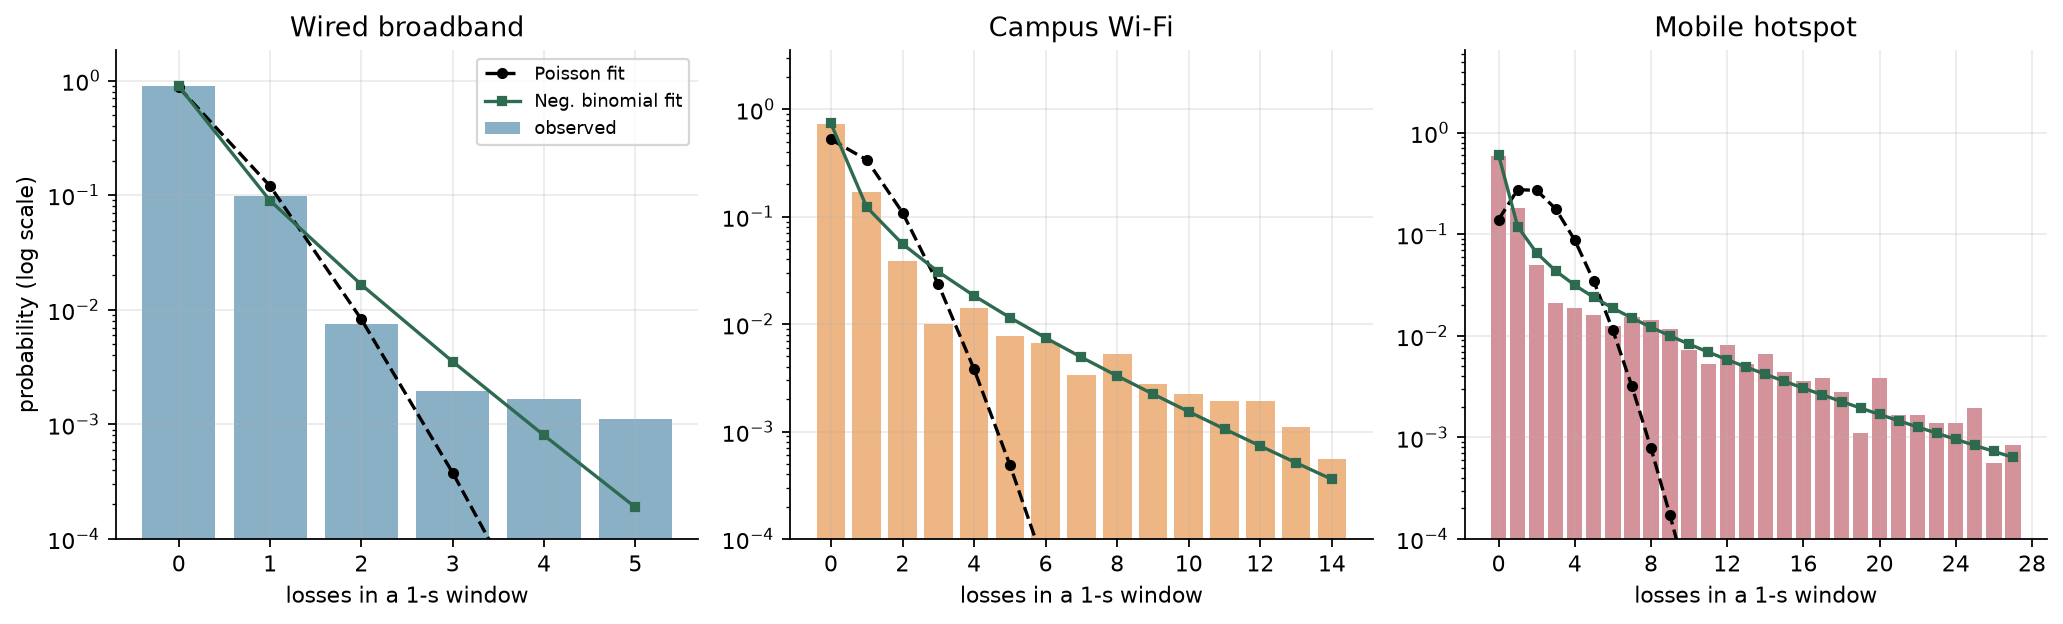
\includegraphics[width=0.92\textwidth]{fig2_count_distribution_fits.png}
\caption{Distribution of losses per second (log scale). The Poisson fit (dashed) falls far below the observed tail. The Negative Binomial (green) follows it.}
\label{fig:counts}
\end{figure*}

\subsection{Inter-loss gaps}
The exponential model is rejected for every network by the bootstrap KS test (Table~\ref{tab:gaps}). Its survival curve is a straight line on a log scale, and the observed curve is not (Fig.~\ref{fig:gaps}). The observed curve drops steeply at first and then flattens. The two-phase mixture captures this shape. Its fast phase has a mean gap of <<fast_lo>> to <<fast_hi>>~ms, about one or two packet intervals, and stands for gaps inside a burst. Its slow phase has a mean of <<M_slows>>~s to <<W_slows>>~s, the spacing between bursts. The fast phase holds <<W_wfast>> of gaps on Wired and <<M_wfast>> on Mobile. The mixture is an adequate fit for Wired ($p=<<W_ksmix>>$) and lowers the AIC sharply for all three networks, although the KS test still detects a misfit for Wi-Fi and Mobile.

\begin{table}[t]
\caption{Inter-loss gaps: exponential and two-phase fits}
\label{tab:gaps}
\centering
\footnotesize
\setlength{\tabcolsep}{3pt}
\begin{tabular}{lccccccc}
\toprule
Net. & $w$ & Fast & Slow & \multicolumn{2}{c}{KS $p$} & \multicolumn{2}{c}{AIC} \\
 & & (ms) & (s) & exp. & mix. & exp. & mix. \\
\midrule
<<rows_gaps>>
\bottomrule
\end{tabular}
\\[2pt]
\raggedright\scriptsize $w$ is the share of gaps in the fast phase. Fast and slow give the mean gap of each phase.
\end{table}

\begin{figure*}[t]
\centering
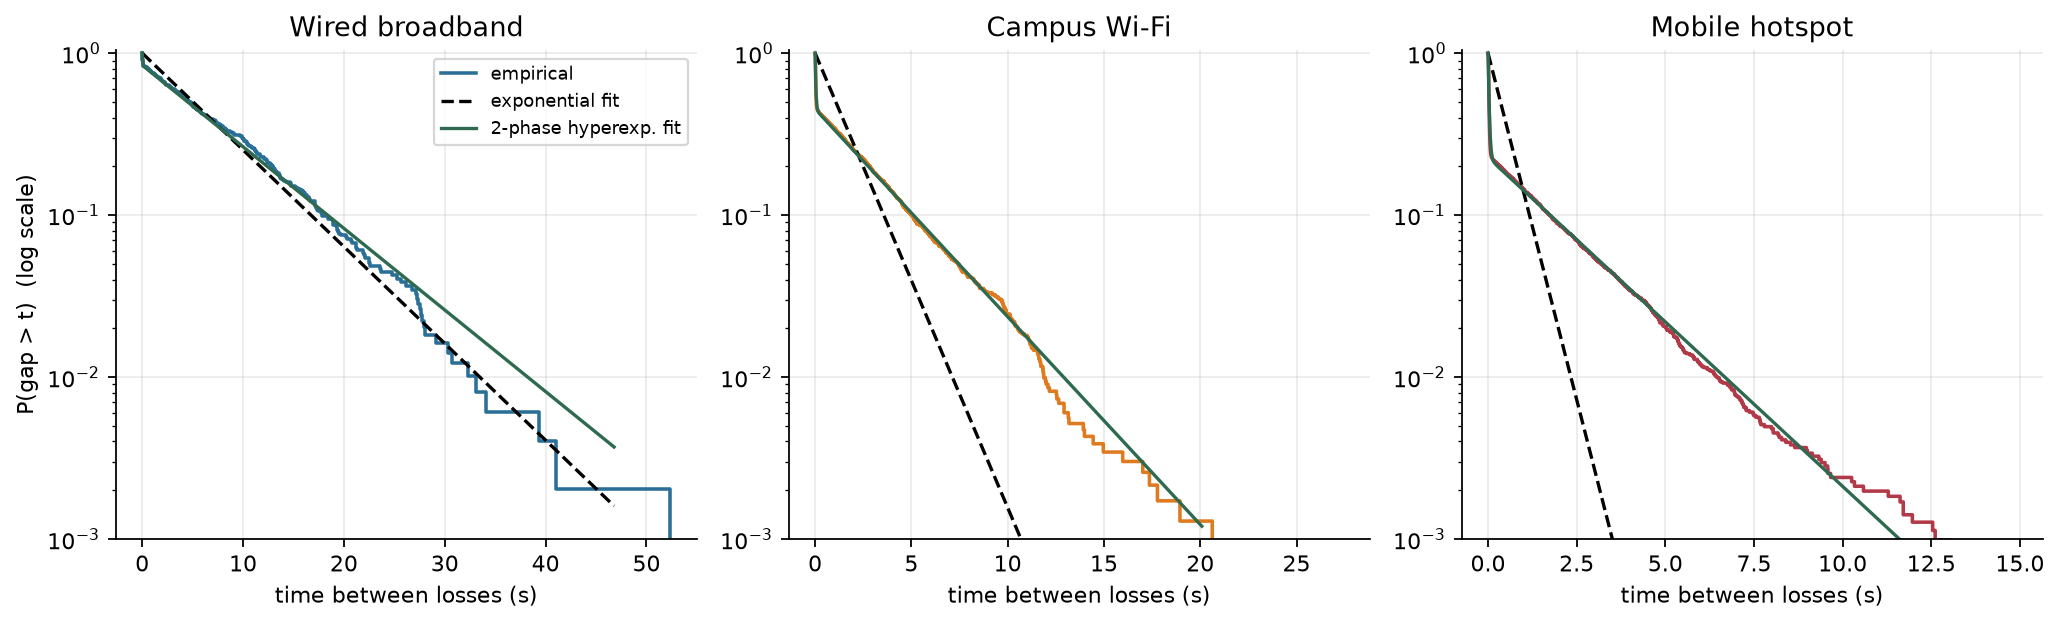
\includegraphics[width=0.92\textwidth]{fig3_gap_survival.png}
\caption{Probability that a gap exceeds $t$ (log scale). An exponential law gives a straight line (dashed). The two-phase mixture (green) follows the observed curve.}
\label{fig:gaps}
\end{figure*}

\subsection{Dependence between packets}
Both independence tests reject $H_0$ with $p<10^{-10}$ for all networks (Table~\ref{tab:dep}). On Wi-Fi there are <<F_runs>> runs where independence predicts <<F_runsE>> ($z=<<F_z>>$). The loss probability after a delivered packet is <<F_a>>, and after a lost packet it is <<F_b>>. The posterior median of $b/a$ is <<list_amp>> for Wired, Wi-Fi and Mobile, so a loss makes the next loss <<amp_lo>> to <<amp_hi>> times more likely (Fig.~\ref{fig:markov}). The posterior probability that $b>a$ is <<pbga>> for every network. The posterior median burst length is <<list_blen>> packets.

\begin{table}[t]
\caption{Tests of independence and burst parameters}
\label{tab:dep}
\centering
\footnotesize
\setlength{\tabcolsep}{2.2pt}
\begin{tabular}{lcccccccc}
\toprule
Net. & Runs & $E[R]$ & $z$ & $G^2$ & $P(L|N)$ & $P(L|L)$ & $b/a$ & Burst \\
\midrule
<<rows_dep>>
\bottomrule
\end{tabular}
\\[2pt]
\raggedright\scriptsize $b/a$ and burst length (packets) are posterior medians. All $p<10^{-10}$.
\end{table}

\begin{figure}[t]
\centering
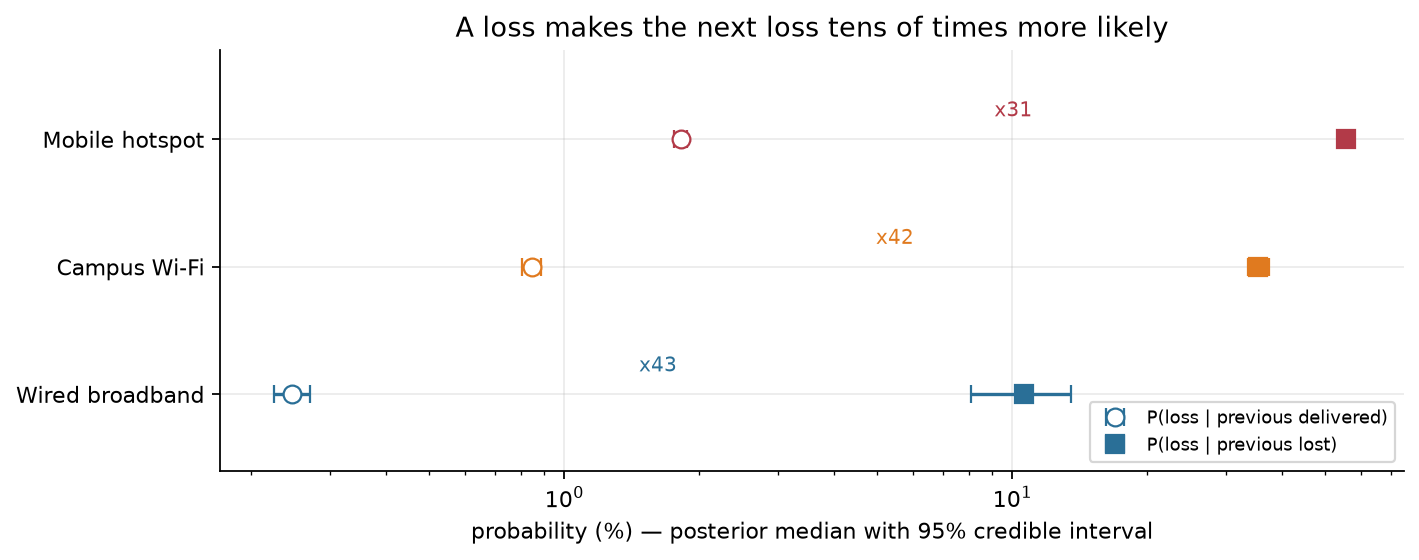
\includegraphics[width=\columnwidth]{fig5_markov_posteriors.png}
\caption{Posterior medians and 95\% credible intervals for $P(L\mid N)$ (open) and $P(L\mid L)$ (filled).}
\label{fig:markov}
\end{figure}

\subsection{Comparison and Bayesian estimates}
The three networks differ clearly. The Kruskal-Wallis statistic is $H=<<kw_H>>$, the $\chi^2$ homogeneity statistic is <<chi_hom>> on <<chi_hom_df>> degrees of freedom, and the largest Bonferroni-corrected pairwise p-value is <<bonf_max>>. The posterior means of the loss rate are <<list_pmean>> (Table~\ref{tab:bayes}), and the posterior probability of the ordering Wired $<$ Wi-Fi $<$ Mobile is <<ordering>>. Sequential updating on <<seq_label>> shows the posterior narrowing from <<seq_first>> after <<seq_first_t>>~s to <<seq_last>> after <<seq_last_t>>~s.

The posterior predictive check exposes the independent model. On Wi-Fi it gives a probability of <<F_pred>> for at least <<heavy_k>> losses in a second, while the observed share is <<F_seen>>, about <<F_ratio>> times higher.

\subsection{Coverage of interval estimates}
Table~\ref{tab:bayes} and Fig.~\ref{fig:coverage} give the result that matters most in practice. Across <<cov_reps>> simulated <<cov_min>>-minute captures, the naive 95\% interval contains the true loss rate in <<list_covN>> of cases. The design effect is <<W_deff>>, <<F_deff>> and <<M_deff>>, so on Wi-Fi the <<packets>> packets carry about as much information as <<F_neff>> independent ones. The adjusted intervals reach <<list_covA>> coverage, close to the nominal level. Their average width grows from <<F_wN>> to <<F_wA>> percentage points on Wi-Fi. In the full Wi-Fi trace the true rate is <<F_true>>. The naive interval <<F_pci>> misses it, while the adjusted interval <<F_aci>> contains it.

\begin{table*}[t]
\caption{Loss-rate estimates and coverage of 95\% intervals}
\label{tab:bayes}
\centering
\footnotesize
\setlength{\tabcolsep}{8pt}
\begin{tabular}{lcccccc}
\toprule
Network & Posterior mean & Naive 95\% interval & deff & Adjusted 95\% interval & Naive coverage & Adjusted coverage \\
\midrule
<<rows_bayes>>
\bottomrule
\end{tabular}
\\[2pt]
\raggedright\scriptsize Intervals are from the full <<duration_h>>-hour trace. Coverage is from <<cov_reps>> simulated <<cov_min>>-minute captures.
\end{table*}

\begin{figure}[t]
\centering
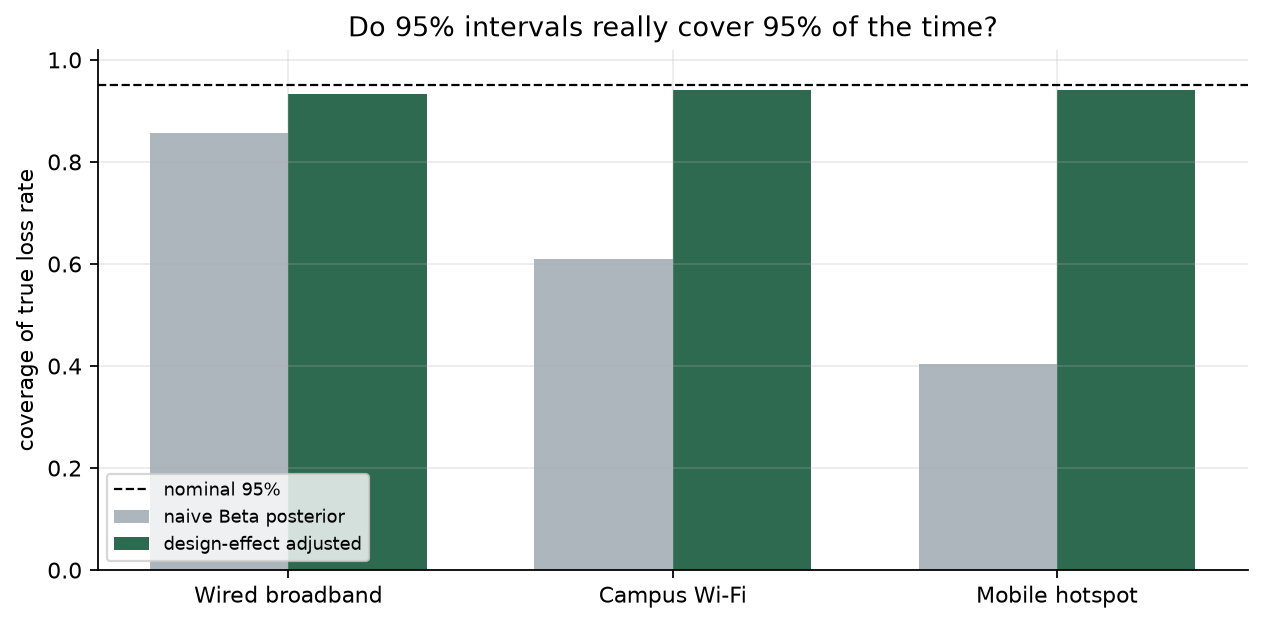
\includegraphics[width=\columnwidth]{fig7_interval_coverage.png}
\caption{Coverage of nominal 95\% intervals for the true loss rate, naive and design-effect adjusted.}
\label{fig:coverage}
\end{figure}

\subsection{Power and capture length}
Fig.~\ref{fig:power} shows the power of the three tests as the capture grows. Table~\ref{tab:power} lists the shortest tested length that reaches a power of <<power_target>>. Mobile needs <<M_pwR>>~s and Wi-Fi <<F_pwR>>~s with the runs test, while Wired needs <<W_pwR>>~s because its bursts are rare and short. The runs test is the most powerful of the three for every network. At <<dur_hi>>~s every test has a power of at least <<min_pw_hi>> on every network, so we recommend captures of at least ten minutes for Phase 2.

\begin{table}[t]
\caption{Shortest capture (s) with power at least <<power_target>>}
\label{tab:power}
\centering
\footnotesize
\begin{tabular}{lcccc}
\toprule
Network & Dispersion & Runs & Markov & Min. power at <<dur_hi>> s \\
\midrule
<<rows_power>>
\bottomrule
\end{tabular}
\end{table}

\begin{figure*}[t]
\centering
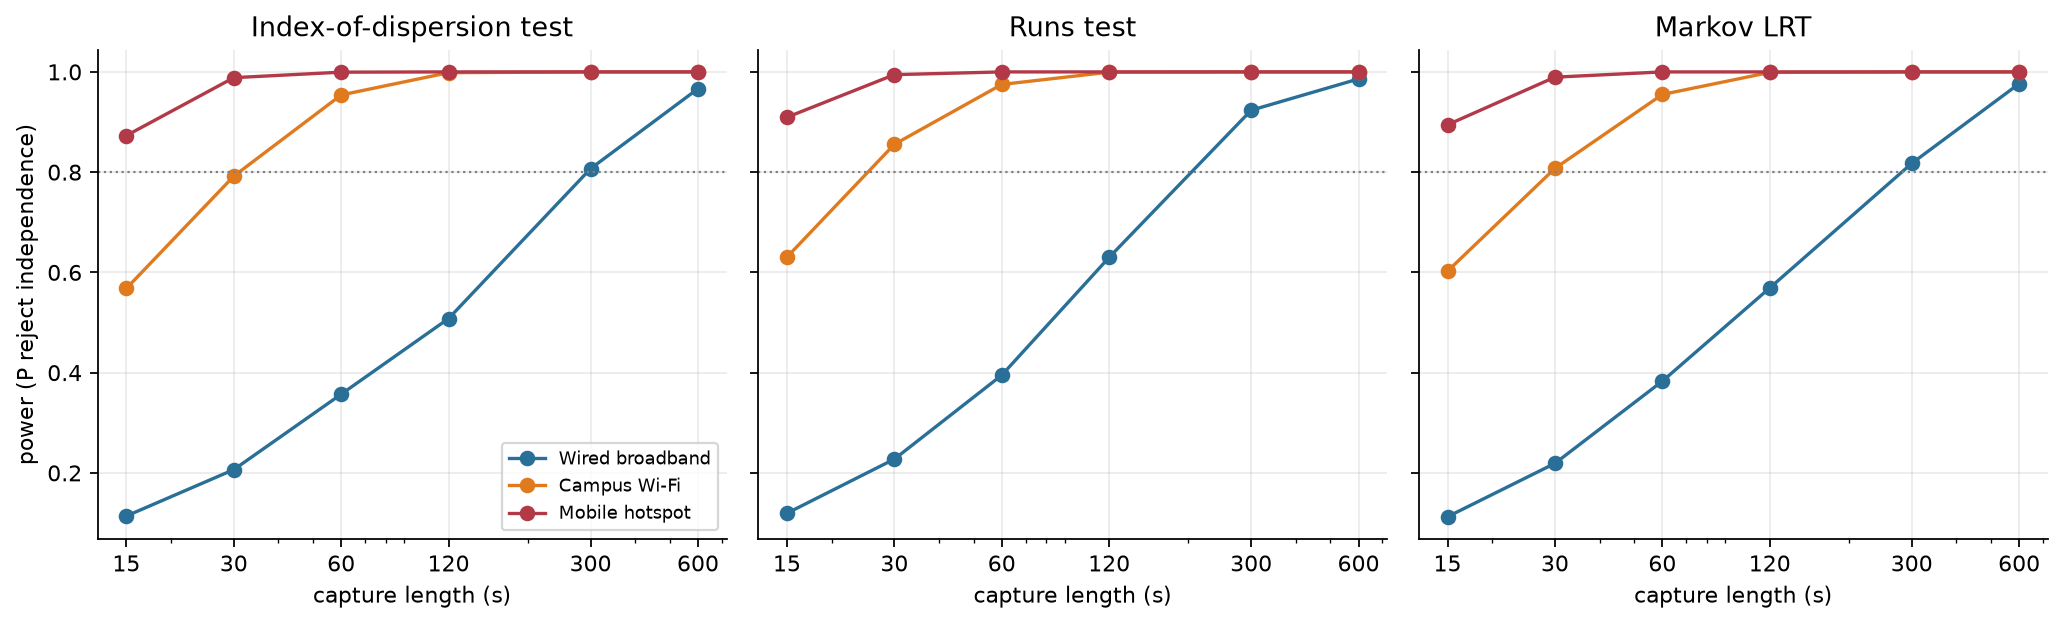
\includegraphics[width=0.92\textwidth]{fig6_power_curves.png}
\caption{Power to reject independence against capture length, from <<power_reps>> simulated captures per point. The dotted line marks a power of 0.8.}
\label{fig:power}
\end{figure*}

\section{Discussion and Limitations}
The results tell one consistent story. A small amount of state, a Bad spell lasting a few packets, is enough to break every model that assumes independence. The loss rate alone hides this. Wired and Mobile differ by a factor of about <<ratio_MW>> in loss rate, but their burst amplification factors are of the same order. Dependence is therefore a separate property of a link and has to be measured on its own.

The coverage study shows why this matters for inference. A naive interval treats every packet as a fresh piece of evidence. When packets inside a burst share their fate, the effective sample is far smaller, and the interval is too narrow. The effect grows with burstiness: Mobile, the burstiest network, has the lowest naive coverage. The design-effect correction is simple and needs only block counts, yet it brings coverage near 95\% in all three cases.

The study has several limitations. First, the data are simulated from the same family of model that motivates the analysis. The tests themselves do not use this knowledge, and the true parameters are used only to judge the estimates, but real links may show other effects such as diurnal load. Phase 2 addresses this. Second, the dispersion test compares the counts with a Poisson law, while counts of <<rate>> packets per window are Binomial with variance slightly below the mean. The test is therefore conservative and does not over-state burstiness. Third, the runs and Markov tests rely on large-sample approximations. Their false-rejection rate in very short captures can move away from 5\%, although it is close to 5\% for hour-long traces. Fourth, the Negative Binomial and the two-phase mixture are still rejected for Wi-Fi and Mobile with large samples, so neither is a complete description. Fifth, the design effect depends on the block length; the <<block_s>>-s blocks used here are much longer than the mean Bad spell. Finally, the results come from one seeded trace per network, although the Monte Carlo studies repeat the process thousands of times.

\section{Conclusion and Future Work}
We tested the independence assumption for packet loss on <<n_scen>> simulated networks. The Poisson and exponential models were rejected in every case. Losses per second were over-dispersed by a factor of <<list_D>>, gaps split into a fast in-burst phase and a slow between-burst phase, and a loss made the next loss <<amp_lo>> to <<amp_hi>> times more likely. Naive 95\% intervals for the loss rate covered the truth in only <<covN_lo>> to <<covN_hi>> of simulated captures, and a design-effect correction raised this to <<covA_lo>> to <<covA_hi>>.

Phase 2 will record constant-rate streams of <<rate>> packets per second on real wired, Wi-Fi and mobile links, for at least ten minutes each, and run the same pipeline. We also plan to estimate the Gilbert-Elliott parameters from real traces with the Baum-Welch algorithm \cite{baum1970}, to test three-phase mixtures and hidden Markov models for the tails, to pool the networks in a hierarchical Bayesian model with the Phase 1 posteriors as priors, and to compare peak and off-peak loss.

\section*{Reproducibility}
All results come from one Python pipeline built on NumPy \cite{numpy2020}, SciPy \cite{scipy2020} and Matplotlib \cite{matplotlib2007}, run with seed <<seed>>. The code is available at \url{https://github.com/AashmanBiyani08/Prob_Stats_Project}.

\IEEEtriggeratref{12}
\begin{thebibliography}{99}
\bibitem{gilbert1960} E. N. Gilbert, ``Capacity of a burst-noise channel,'' \emph{Bell Syst. Tech. J.}, vol. 39, no. 5, pp. 1253-1265, 1960.
\bibitem{elliott1963} E. O. Elliott, ``Estimates of error rates for codes on burst-noise channels,'' \emph{Bell Syst. Tech. J.}, vol. 42, no. 5, pp. 1977-1997, 1963.
\bibitem{bolot1993} J.-C. Bolot, ``End-to-end packet delay and loss behavior in the Internet,'' in \emph{Proc. ACM SIGCOMM}, 1993, pp. 289-298.
\bibitem{paxson1997} V. Paxson, ``End-to-end Internet packet dynamics,'' in \emph{Proc. ACM SIGCOMM}, 1997, pp. 139-152.
\bibitem{yajnik1999} M. Yajnik, S. Moon, J. Kurose, and D. Towsley, ``Measurement and modelling of the temporal dependence in packet loss,'' in \emph{Proc. IEEE INFOCOM}, 1999, pp. 345-352.
\bibitem{jiang2000} W. Jiang and H. Schulzrinne, ``Modeling of packet loss and delay and their effect on real-time multimedia service quality,'' in \emph{Proc. NOSSDAV}, 2000.
\bibitem{hasslinger2008} G. Hasslinger and O. Hohlfeld, ``The Gilbert-Elliott model for packet loss in real time services on the Internet,'' in \emph{Proc. 14th GI/ITG Conf. Measurement, Modelling and Evaluation of Computer and Communication Systems (MMB)}, 2008, pp. 269-286.
\bibitem{dempster1977} A. P. Dempster, N. M. Laird, and D. B. Rubin, ``Maximum likelihood from incomplete data via the EM algorithm,'' \emph{J. Roy. Statist. Soc. B}, vol. 39, no. 1, pp. 1-38, 1977.
\bibitem{akaike1974} H. Akaike, ``A new look at the statistical model identification,'' \emph{IEEE Trans. Autom. Control}, vol. 19, no. 6, pp. 716-723, 1974.
\bibitem{lilliefors1969} H. W. Lilliefors, ``On the Kolmogorov-Smirnov test for the exponential distribution with mean unknown,'' \emph{J. Amer. Statist. Assoc.}, vol. 64, pp. 387-389, 1969.
\bibitem{efron1993} B. Efron and R. J. Tibshirani, \emph{An Introduction to the Bootstrap}. New York: Chapman \& Hall, 1993.
\bibitem{wald1940} A. Wald and J. Wolfowitz, ``On a test whether two samples are from the same population,'' \emph{Ann. Math. Statist.}, vol. 11, no. 2, pp. 147-162, 1940.
\bibitem{wilks1938} S. S. Wilks, ``The large-sample distribution of the likelihood ratio for testing composite hypotheses,'' \emph{Ann. Math. Statist.}, vol. 9, no. 1, pp. 60-62, 1938.
\bibitem{kruskal1952} W. H. Kruskal and W. A. Wallis, ``Use of ranks in one-criterion variance analysis,'' \emph{J. Amer. Statist. Assoc.}, vol. 47, pp. 583-621, 1952.
\bibitem{mann1947} H. B. Mann and D. R. Whitney, ``On a test of whether one of two random variables is stochastically larger than the other,'' \emph{Ann. Math. Statist.}, vol. 18, no. 1, pp. 50-60, 1947.
\bibitem{kish1965} L. Kish, \emph{Survey Sampling}. New York: Wiley, 1965.
\bibitem{gelman2013} A. Gelman, J. B. Carlin, H. S. Stern, D. B. Dunson, A. Vehtari, and D. B. Rubin, \emph{Bayesian Data Analysis}, 3rd ed. Boca Raton, FL: CRC Press, 2013.
\bibitem{baum1970} L. E. Baum, T. Petrie, G. Soules, and N. Weiss, ``A maximization technique occurring in the statistical analysis of probabilistic functions of Markov chains,'' \emph{Ann. Math. Statist.}, vol. 41, no. 1, pp. 164-171, 1970.
\bibitem{numpy2020} C. R. Harris \emph{et al.}, ``Array programming with NumPy,'' \emph{Nature}, vol. 585, pp. 357-362, 2020.
\bibitem{scipy2020} P. Virtanen \emph{et al.}, ``SciPy 1.0: Fundamental algorithms for scientific computing in Python,'' \emph{Nature Methods}, vol. 17, pp. 261-272, 2020.
\bibitem{matplotlib2007} J. D. Hunter, ``Matplotlib: A 2D graphics environment,'' \emph{Comput. Sci. Eng.}, vol. 9, no. 3, pp. 90-95, 2007.
\end{thebibliography}

\end{document}
